\documentclass[main.tex]{subfiles}

\begin{document}

\section*{Goal}
This week we will preform three different activities to learn about the relationship of position, velocity, and acceleration. We will start with looking at two different ways to calculate the acceleration due to gravity, then finish with an experiment using a motor to accelerate the cart.

\section*{Equipment}
\begin{itemize}
\item
850 Universal Interface (850UI)
\item
PASCO Capstone
\item
Motion Sensor, Photogate
\item
Low-friction track, regular cart, fan cart, and support rod
\item
Large picket fence
\item
Meter stick
\end{itemize}

\section*{Theory}
We can describe the position of an object, given a constant acceleration, $a$, by the following equation,
\begin{equation} \label{eq:pos}
x=x_0+v_0 t+\frac{1}{2}at^2,
\end{equation}
where $x_0$ and $v_0$ are the initial position and velocity respectively. We can identify this equation as quadratic equation.

If we were to take the derivative of Equation~\eqref{eq:pos} with respect to time we would get,
\begin{equation} \label{eq:vel}
\frac{d}{dt}x=v=v_0+at,
\end{equation}
which is another of the kinematic equations that describes the velocity of an object under acceleration.

Finally, if we take the derivative of Equation~\eqref{eq:vel} or equivalently, the second derivative of Equation~\eqref{eq:pos} we have,
\begin{equation} \label{eq:acc}
\frac{dv}{dt}=\frac{d^2 x}{dt^2}=a.
\end{equation}

For those without any prior exposure to calculus, don't panic!  All we need to know is that a derivative is an equation that defines the slope of a curve at a single point. Thus, the second derivative is simply the ``slope of the slope" and so on.

For a freely-falling object the acceleration experienced will be due to the gravitational force. We give this acceleration a special symbol,$g,$ as it is the same value everywhere near the surface of Earth, $g=9.81\text{ m/s}^2.$ As acceleration is a vector, and since the vertical direction going upward is normally taken as positive, we often use a negative sign with $g$ to indicate that the acceleration is downward.

\section{Setup I: Acceleration on a freely-falling body}
\begin{center}
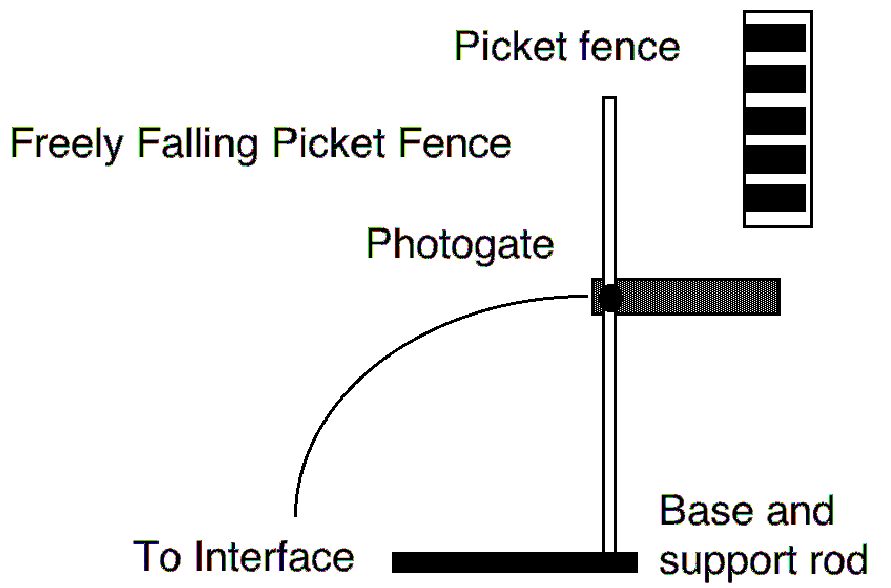
\includegraphics[width=0.5\textwidth]{Accel_1_Setup}
\end{center}
\begin{enumerate}
\item
Attach the Photogate to digital channel 1. Setup the Photogate at the edge of the table so that the regular picket fence can pass through as shown. 
\item
Open Capstone.
\item
Under ``Hardware Setup" in the toolbar on the left, click on digital channel 1 on the picture of the 850UI and add a Photogate. You can do this by scrolling through the list and clicking or by typing ``Photogate" into the search bar. Note: We want \emph{``Photogate"} not ``Photogate with Pulley."
\item
There will now be a new button in the toolbar on the left called ``Timer Setup." We need to tell Capstone how the Photogate will be used.
\item
Click on ``Timer Setup" and follow the on-screen instructions to setup a Pre-Configured Timer for Photogate, Ch 1. On step 3 of the timer, choose ``Picket Fence." Make sure that ``Speed," ``Acceleration," and ``Position" are all checked. Finally, make sure the Flag Spacing is set to 0.05 m. Click ``Finish" to complete the timer setup. Click on ``Timer Setup" to hide the window.
\item
We want to create a graph for our experiment. To do this, double-click on the button labeled ``Graph" in the toolbar on the right.
\item\label{step:accel_add_position}
To tell Capstone what data to plot, click on the ``\textless Select Measurement\textgreater" button on the vertical axis and select ``Position."
\item
We want to also show velocity and acceleration on the same graph. To do this in the toolbar above the graph, click on this button 
\includegraphics{Add_New_Plot} twice.
 This will add two graphs below our current one.
\item
Repeat the process from Step~\ref{step:accel_add_position} to select ``Speed" and ``Acceleration."
\end{enumerate}

\subsection*{Procedure}
\begin{enumerate}
\item
Click on the Record button at the bottom. Capstone will begin data collection when the Photogate is first blocked.
\item
Do not let the picket fence hit the floor. Put a book bag, coat or other soft object underneath the Photogate so that the picket fence doesn't break.
\item
Drop the regular picket fence through the Photogate. Click Stop in the toolbar. If the picket fence hits the Photogate, then do it again. When you have a good run hide any ``bad" data runs, so that you only see the good one. Press the Scale to fit button 
\includegraphics{Rescale}. n.b., how you rescaled graph looks may depend on which graph panel (there are 3 here) is active at a time. Experiment with clicking on one panel (say, Position vs. Time) and then clicking on the Scale to Fit button. Repeat with each panel. Which should you choose? Choose the one that shows all of the data in all 3 panels.
\end{enumerate}

\subsection*{Analysis}
\begin{enumerate}
\item
Click on the Position versus Time graph. Fit the data 
\includegraphics{Curve_Fit} with a Quadratic Fit. You can move the fit info box around so that it does not obscure the data. The A value is the quadratic coefficient, B the linear coefficient, and C the constant term. Comparison with Equation~\eqref{eq:pos} will show you what each of these coefficients correspond to. 
\item
Click on the Speed versus Time graph. Fit the data with a Linear Fit. 
\item
Click on the Acceleration versus Time graph. Calculate the mean and standard deviation of the data by selecting the Statistics button, 
\includegraphics{Statistics} in the graph toolbar and choosing those options. Uncheck Maximum and Minimum options. Click the $\Sigma$ to make the results show on the graph. 
\item
\textbf{Print} a copy of this graph for each member of the group.
\item
Using the results from all three graphs, compare the experimental values to the standard value of $g$ using a percent discrepancy.
\end{enumerate}

\begin{question}
From the step above which graph gives the best value of $g$? Which is the worst? Why?
\end{question}
\begin{question}
The experiment indicates that the acceleration due to gravity is a positive number, not a negative. What is the significance of this? Does it matter?
\end{question}

\section{Setup II: Acceleration on an inclined plane.}
In this experiment, we will again be determining $g.$ However, instead of just dropping an object, let's roll a cart down a track. In this situation, the acceleration of the cart will be actually slower than if it were just falling. The acceleration of the cart will be,
\begin{equation}\label{eq:AsinG}
a=g\sin{\theta},
\end{equation}
where $\theta$ is the angle the track makes with the table. 

\begin{enumerate}
\item
Remove any extraneous equipment from earlier activities, wrap the cords and put aside.

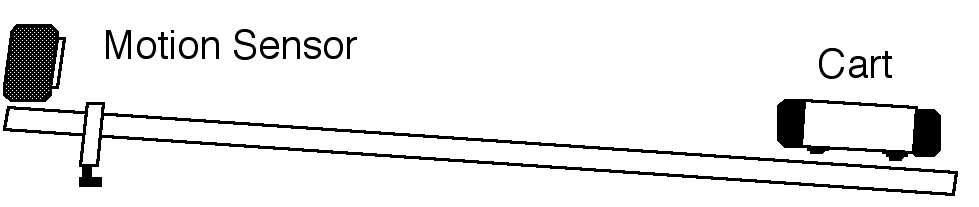
\includegraphics[width=\textwidth]{Accel_2_Setup}
\item
Position the Motion sensor on the dynamics track as shown. Plug the Motion sensor into the 850UI.
\item
Choose ``New Activity" from the File menu in Capstone. Answer ``Discard" when asked to save the previous activity.
\item
Under ``Hardware Setup" add the Motion Sensor to the appropriate ports.
\item
Double-click the Graph icon in the toolbar on the right.
\item
Create a three-paneled graph as we did in Setup I for Position, Velocity, and Acceleration. 
\end{enumerate}•

\subsection*{Procedure}
\begin{enumerate}
\item
Calculate the angle of the inclined track. We can do this by measuring the height of the track and the length of the track and using the following trigonometric definition to find the angle,
\[
\theta=\arcsin\left(\frac{Height}{Length}\right).
\]
To get an accurate value of the angle, make sure to measure the height of the bottom surface of the track, not the top surface.
\item
Position the Motion sensor at the high end of the track. The cart will start at the low end of the track and be pushed up toward the motion sensor.
\item
Before recording any data for later analysis, you should experiment with the motion sensor to make sure it is aligned and can ``see" the cart as it moves.
\item
Place the cart on the low end of the track (i.e., the end opposite to the motion sensor).
\item
Click the Record button to begin recording data. 
\item
Give the cart a firm push up the track so the cart will move up the inclined plane toward and then away from the motion sensor. Don't push the cart so firmly that it gets closer than 15 cm to the sensor. Continue collecting data until the cart has returned to the bottom of the track. Click the Stop button to end data recording. (If the data points do not appear on the graph or do not form a smooth graph, check the alignment of the motion sensor, remove the bad data, and try again.)
\item
Click the Scale To Fit button to automatically rescale the Graph.
\end{enumerate}

\subsection*{Analysis}
\begin{enumerate}
\item
Click the mouse in the ``Velocity vs. Time" panel of the graph.
\item
Choose a linear fit to the graph. The slope of this line is the average acceleration.
\item
In the plot of velocity, use the Selection Tool, 
\includegraphics{Selection_Tool} to select the points of the plot that shows the cart's motion after the push and before it stopped at the bottom of the track. This will force Capstone to only use the points within the box in calculating the fit of the line.
\item
Click the mouse in the ``Acceleration vs. Time" panel of the graph.
\item
In the plot of acceleration, use the Selection Tool to include only the region of the plot that corresponds to the cart's motion after the push and before it stopped at the bottom of the track. Record the mean of the acceleration.
\item
Click on the triangle to the right of the Show Selected Statistics button 
\includegraphics{Statistics}. Check the ``Mean" and ``Standard Deviation" choices and uncheck everything else. Finally click the $\Sigma$ to actually display the information. 
\item
\textbf{Print} a copy of this graph for each member of your lab table.
\item \label{step:TheoA}
Calculate the theoretical value for the acceleration of the cart using Equation~\eqref{eq:AsinG} and $g=9.81 \text{ m/s}^2.$
\end{enumerate}•

\begin{question}
Describe the position versus time plot of the Graph display. Why does the distance begin at a maximum and decrease as the cart moves up the inclined plane?
\end{question}
\begin{question}
By averaging the results of both the Velocity vs. Time and the Acceleration vs. Time plots, calculate the percent discrepancy using the theoretical value from Analysis step~\ref{step:TheoA}.
\end{question}
\begin{question}
If the mass of the cart is doubled, how should the results be affected? Explain.
\end{question}

\section{Setup III: Acceleration from a fan.}
For this last activity we will NOT be using the acceleration due to gravity, but instead the acceleration provided by a Fan Cart. We shall compare the position, velocity and acceleration data of the fan cart with Equations~\eqref{eq:pos},~\eqref{eq:vel}, and~\eqref{eq:acc}.

\subsection*{Procedure}
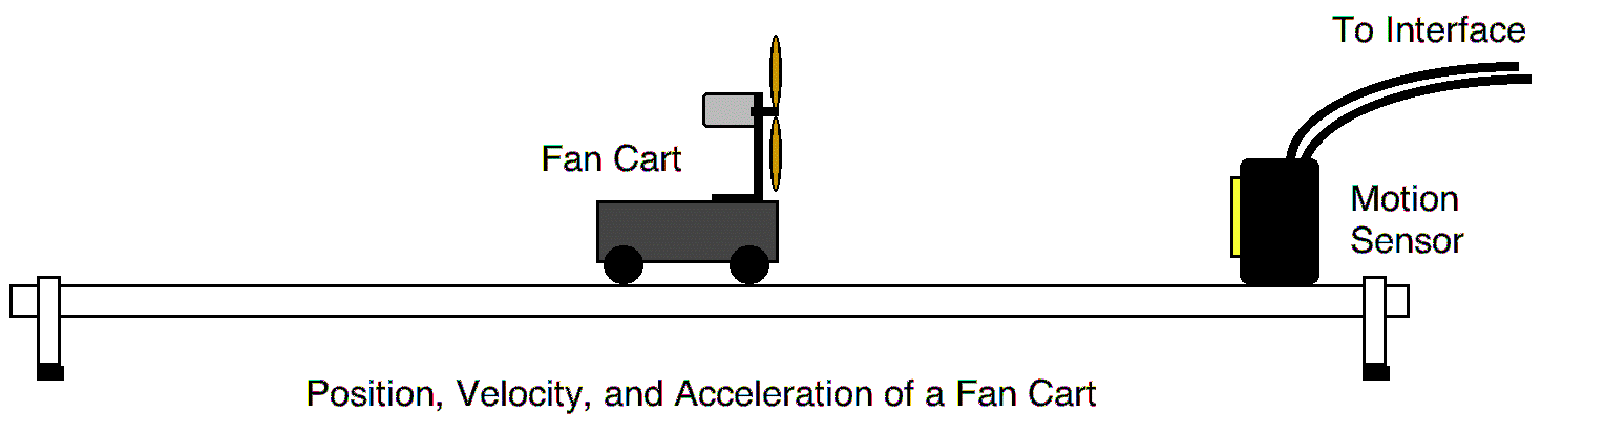
\includegraphics[width=\textwidth]{Accel_3_Setup}
\begin{enumerate}
\item
Arrange the Fan Cart, Motion Sensor, and track as shown. Tie a string to the fan cart so that we can hold the fan cart before releasing it without interfering with the motion sensor.
\item
We will use the same graph configuration as we did in Setup II. However, make sure that all of the previous data runs have been deleted.
\item
Hold the string so that the fan cart remains stationary about 40 cm in front of the Motion Sensor. Also, make sure that the fan cart is pulling away from the motion sensor!
\item
Click on ``Record" to begin data collection.
\item
Release the fan cart.
\item
When the cart has traveled the length of the available track, click ``Stop" to finish data collection.
\end{enumerate}•

\subsection*{Analysis}
\begin{enumerate}
\item
Scale your data to best fit your graph window.
\item \label{step:select}
Click on the Selection Tool, 
\includegraphics{Selection_Tool}. Drag and resize the box to only include a relatively small region of the Position vs. Time plot that shows a smooth parabolic curve. Try to include about five or six data points in the box.
\item
Press Scale to fit, 
\includegraphics{Rescale}. This will rescale all three graphs so that they display the same time interval. If you are not satisfied with your selection, right-click in the selection box, and click ``Delete Highlighter," press the Scale to fit button again, then repeat step~~\ref{step:select}.
\item
Click on the Position vs. Time graph. Fit the data with a Quadratic Fit. You can move the fit info box around so that it does not obscure the data. The $A$ value is the quadratic coefficient, $B$ the linear coefficient, and $C$ the constant term.
\item
Click on the Velocity versus Time graph. Fit the data with a Linear Fit.
\item
Click on the Acceleration versus Time graph. Calculate the mean and standard deviation of the data by selecting the Statistics triangle 
\includegraphics{Statistics} in the graph toolbar and choosing those options.
\item
\textbf{Print} this graph for all group members.
\item
Identify the value of $a$ from each of the three graphs using the appropriate results from the curve fits.
\end{enumerate}•

\begin{question}
Calculate the percent discrepancy of each of the two other accelerations using the mean from the Acceleration vs. Time graph as the standard. 
\end{question}

\begin{samepage}
\hrulefill\\ \\
\emph{Chapter~\ref{chap:Acceleration}:} \textbf{Acceleration}
\begin{enumerate}
\item
\textbf{(1)} Title page --- title, your name, name of lab partners, date of lab.
\item
\textbf{(5)} Purpose --- What was the goal of Acceleration II?
\item
\textbf{(12)} Theory --- Show how Equations~\eqref{eq:pos},~\eqref{eq:vel}, and~\eqref{eq:acc} are related. If you are in Algebra-based physics, talk about slopes. If you are in Calculus-based physics, use derivatives. What shape should the position, velocity, and acceleration graphs have for freely falling objects?
\item
\textbf{(3)} Data Table 
\item
\textbf{(6)} All graphs. There are 3 of them.
\item
\textbf{(6)} Calculations --- Show calculations e.g., percent discrepancies, theoretical values
\item
\textbf{(12)} Answer all questions.
\item
\textbf{(5)} Conclusion --- What were your findings from Acceleration II? Explain.
\end{enumerate}•
\end{samepage}

\newpage
\section{Data Table}
\subsection*{Setup II}
\begin{doublespace}
\resizebox{0.8\textwidth}{!}{
\begin{tabular}{|l|@{\hskip 2 cm}r|}
\hline
Item & Value\\
\hline
Angle of track & degrees\\
\hline
Acceleration (slope) & $m/s^2$\\
\hline
Acceleration (mean) & $m/s^2$\\
\hline
Acceleration (theoretical) & $m/s^2$\\
\hline
\end{tabular}•
}
\end{doublespace}


\end{document}
